
\chapter{Solar wind and CME influence on geomagnetic activity}
\label{chap:chapter2}

%context
Variations in the Earth's magnetosphere are largely evoked by influence through the solar wind. These magnetospheric disturbances have diverse effects on the terrestrial environment. Especially the effects of severe geomagnetic storms created by coronal mass ejections (CMEs) pose various threats to sensitive technical systems and exposed humans. Thus, the development of quantitative forecasts for magnetospheric impacts caused by solar wind and CMEs is of major importance.
The analyses in this chapter are based on my work done for the EU~FP7 project Advanced Forecast For Ensuring Communications Through Space (AFFECTS) which ran from 2011 to 2013.

%aims
The goals of this study are to estimate the magnetospheric impact from solar wind and also to predict it for remotely forecasted CMEs and streams in particular. Empirical dependencies between the solar wind and the magnetospheric disturbance index~\Kp{} are presented. These relations allow nowcasts from upstream solar wind in-situ measurements and allow forecasts from remote observations of the corona. The \Kp{} nowcast is derived via a relation with the solar wind electric field. The \Kp{} forecasts are based on solar wind velocity and split into CME and stream forecasts. The magnetospheric impact of CMEs is estimated solely based on their arrival velocities which can be predicted from coronagraph observations. The prediction of solar wind stream velocities, e.g., obtained from coronal hole observations, enables to estimate their impact as well.

% data
The solar wind data considered in these analyses consists of 35~years (1981--2016) of high-resolution minutely OMNI data, which is composed of multi-spacecraft intercalibrated in-situ measurements from \SI{1}{\au}. I analyze the \Kp{} frequency distributions with respect to the depending parameters electric field and velocity and compile functional dependencies via logarithmic fitting.
%methods
In order to nowcast the \Kp~index from general solar wind conditions, I apply a correlation with the solar wind electric field -- the product of the parameters velocity and magnetic field z-component in GSM coordinates: $E = - v B_\text{z}$. The solar wind data processing of 3"~hour extreme values is evaluated against 3"~hour averages via the correlation with \Kp{}. A suitable logarithmic function is constructed and its fit to the data results in a functional relation between E"~field and \Kp{}.

Remote solar observations provide enhanced forecast lead times for CMEs and for streams, however, this benefit comes with major limitations on the predicted magnetic field and plasma parameters. The velocity and the direction of CMEs can still be determined in their early near-Sun stages via remote tracking with coronagraph white-light observations. Using these parameters as input for CME propagation models, their possible arrival time and arrival velocity at Earth can be derived, see \autoref{sec:solar_wind_nowcast_and_forecast_to_earth}. Similarly, the Earth arrival time and velocity of solar wind streams can be estimated remotely. Images of the solar surface and the corona reveal the distinct sources of solar wind and indicate the emitted type of solar wind and its properties.

For the purpose of forecasting the \Kp~index from estimated CME and stream velocities, I furthermore filter the solar wind data, using flagged CME times from the solar wind structures (SWS) list provided by \citet{Richardson2012}. Logarithmic fits to the data yield in separate \Kp{} relations for CMEs and streams.
Eventually, I evaluate the prediction performances of the derived relations by analyzing their forecast errors and comparing their true skill statistic.

%%% synopsis
The objectives of the analyses performed and presented in this chapter are to estimate the geomagnetic impact of solar wind and to predict it for CMEs and streams in particular. The analyses are ordered as follows: In \autoref{sec:kp_long_term_variations} I determine the magnitudes of the long-term \Kp{} changes due to solar activity and I measure the extent of seasonal variations stemming from the Earth's orbit. In \autoref{sec:relation_between_sw_efield_and_kp} in order to nowcast the \Kp~index, I quantify the solar wind influence on \Kp{} by deriving a functional relation with the solar wind E"~field. In \autoref{sec:relations_between_cme_stream_v_and_kp} for the purpose of enabling \Kp{} forecasts from remote observations, I estimate the \Kp{} impact coming from CMEs and streams separately by deriving functional dependencies with their velocities. In \autoref{sec:prediction_performance}, the obtained \Kp{} relations are evaluated for their prediction performance. Finally in \autoref{sec:discussion_ch2}, the results are further discussed and at the end of this chapter in \autoref{sec:conclusions_ch2}, the conclusions are presented.


\section{The \Kp{}~index and its long-term variations}
\label{sec:kp_long_term_variations}
% data
The \Kp~index is designed to measure solar particle radiation by its magnetic effects. I use this magnetospheric disturbance index to correlate it with near-Earth solar wind measurements. More detailed information on the \Kp{}~index can be found in \autoref{sec:kp_index}.
The \Kp{} data is obtained from the GFZ~Potsdam, where the index is currently maintained\footnote{GFZ~Potsdam \Kp~index website: \urlfoot{http://www.gfz-potsdam.de/en/kp-index/}}. It covers the time period 1932--2016, see also \autoref{sec:kp_data}. Its frequency distribution shows that the highest frequencies occur around low \Kp{} values of 1+, see \autoref{fig:Kp_histogram_b}. Going to higher \Kp{} values, the frequencies decline asymptotically towards zero -- a \Kp{} value of 9o occurred only 29 times in this time interval.
\begin{figure}[htb]
	\begin{floatrow}
		\ffigbox{
			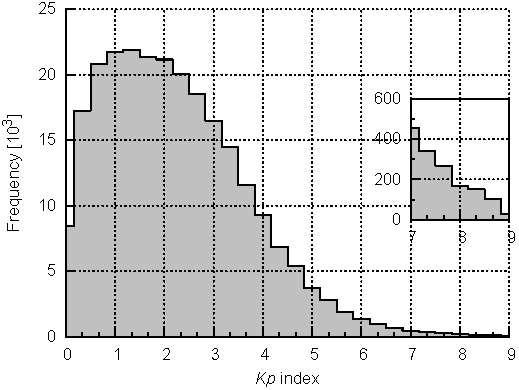
\includegraphics[width=0.46\textwidth]{figures_of_mine/chapter2/Kp_histogram_b.pdf}
		}{
			\caption[\lofimage{figures_of_mine/chapter2/Kp_histogram_b.pdf}I created the figure myself.]
			{\Kp{} frequency distribution for the time period 1932--2016. The inset shows a zoomed-in view of the high-value tail. The \Kp{} data is obtained from the GFZ~Potsdam.}
			\label{fig:Kp_histogram_b}
		}
		\ffigbox{
			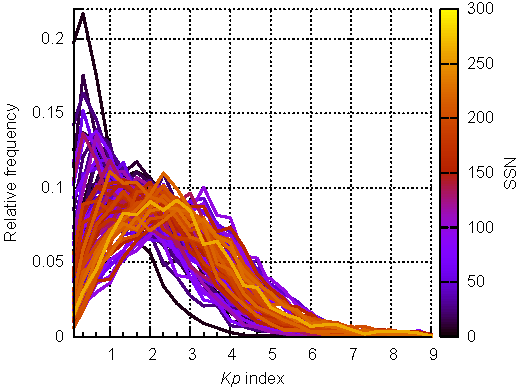
\includegraphics[width=0.95\Xhsize]{figures_of_mine/chapter2/Kp_histogram_yearlySSN_b.pdf}
		}{
			\caption[\lofimage{figures_of_mine/chapter2/Kp_histogram_yearlySSN_b.pdf}I created the figure myself.]
			{Yearly \Kp{} frequency distributions during the period 1932--2016, sorted and colored by yearly SSN. All distributions are normed to be of equal area. The \Kp{} data is obtained from the GFZ~Potsdam and the yearly SSN data from the SILSO World Data Center.}
			\label{fig:Kp_histogram_yearlySSN_b}
		}
	\end{floatrow}
\end{figure}

% intro
As magnetospheric activity is driven by the approaching solar wind, it also reflects the solar wind's long-term variations. The long-term variations of \Kp{} originate from the change in solar activity and the changes due to the Earth's orbit around the Sun. In the following the influence of both effects is quantified. I estimate the long-term variations of the \Kp~index which are contributed by solar activity and seasonal effects.

\subsection{Solar activity influence}
The general \Kp{} distribution seen in \autoref{fig:Kp_histogram_b} averages over solar activity. Lower solar activity comes with a weaker ambient heliospheric magnetic field resulting in weaker geomagnetic activity as well. Solar activity is generally tracked with the international sunspot number (SSN). A functional dependency of the average yearly \Kp~index on the yearly SSN is derived. SSN data from the time period 1917--2016 is used in the present analyses. The data is obtained from the International Sunspot Number Monthly Bulletin and online catalog provided by the WDC-SILSO\footnote{WDC-SILSO website: \urlfoot{http://www.sidc.be/silso/}} at the SIDC (ROB).

The \Kp{} frequency distributions' shape varies with solar activity as is visible in the yearly distributions, sorted and colored by yearly SSN in \autoref{fig:Kp_histogram_yearlySSN_b}. The distribution's peak position scales with SSN, that is, a high yearly SSN results in a higher abundance of large \Kp{} values as well.

The time series of yearly average \Kp{} values from the years 1932--2016 shows a solar cycle imprint, see the top graphs in \autoref{fig:yearly_kp-ssn_correlation_c}.
\begin{figure}
	\fcapside[\FBwidth]{
		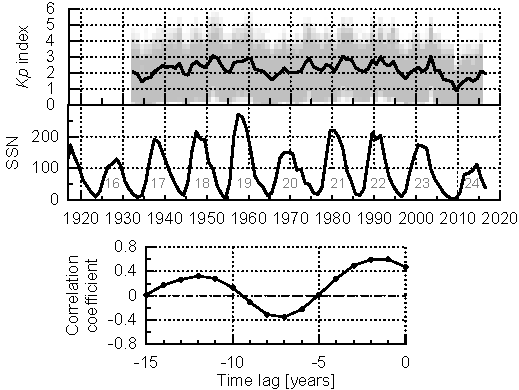
\includegraphics[width=0.6\textwidth]{figures_of_mine/chapter2/yearly_kp-ssn_correlation_c.pdf}
	}{
		\caption[\lofimage{figures_of_mine/chapter2/yearly_kp-ssn_correlation_c.pdf}I created the figure myself.]
		{Yearly \Kp~index distributions (shaded area) with their mean values for the time period 1932--2016 and yearly SSN with cycle number for the time period 1917--2016 (top panels). The Pearson correlation coefficients with the yearly SSN are calculated for time lags back to \num{-15}~years (bottom panel). The \Kp{} data is obtained from the GFZ~Potsdam and the yearly SSN data from the SILSO World Data Center.}
		\label{fig:yearly_kp-ssn_correlation_c}
	}
\end{figure}
The \Kp{} pattern follows the solar cycle minima and maxima as well as the changes in magnitude between solar cycles. The yearly mean \Kp{} shifts about 1~\Kp~unit for both variations separately. As expected, the correlation with solar activity shows an 11-year period, see bottom graph in \autoref{fig:yearly_kp-ssn_correlation_c}. The highest correlation coefficient of 0.60 is found with a time lag of $-1$~year, that is, the yearly average \Kp{} follows the SSN of the previous year.
%Kp-ssn cc: 0.5971

The yearly mean \Kp~index with respect to the 1-year lagged SSN shows a rise with increasing SSN, as seen from \autoref{fig:Kp_SSN_fit_d}.
\begin{figure}
	\fcapside[\FBwidth]{
		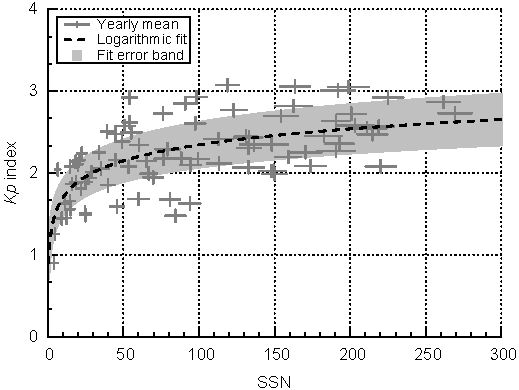
\includegraphics[width=0.6\textwidth]{figures_of_mine/chapter2/Kp_SSN_fit_d.pdf}
	}{
		\caption[\lofimage{figures_of_mine/chapter2/Kp_SSN_fit_d.pdf}I created the figure myself.]
		{Yearly mean \Kp~index with respect to 1-year lagged SSN (+) with the weighted logarithmic fit (dashed line). The error bars denote the SSN standard deviation and the relative weight from the yearly data coverage. The shaded area represents the fit error band derived from the estimated standard deviations of the fit parameters. The logarithmic function (\autoref{eq:log_fit_function}) is used for the weighted fit. The yearly \Kp{} mean values are calculated from GFZ~Potsdam data and the yearly SSN is obtained from the SILSO World Data Center.}
		\label{fig:Kp_SSN_fit_d}
	}
\end{figure}
In order to obtain an analytical relation for this dependency, I perform a least-squares regression fit. \Kp{} itself is a quasi-logarithmic index, so it is apparent to use a logarithmic fit function:
\begin{align}
	f(x) = a \cdot \ln(x) + b	\,.	\label{eq:log_fit_function}
\end{align}
The resulting fit parameters are $a = 0.281(43)$ and $b = 1.05(19)$; the numbers in parentheses are the estimated standard deviations. Concerning the error notation in this work, I adhere to the parentheses notation documented in the ``Guide to the expression of uncertainty in measurement'' (GUM) published by \citet{GUM2008}, where the numbers in parentheses are the errors on the corresponding last digits of the quoted value.

The fit parameters lead to the relation
\begin{align}
	\Kp(ssn) = 0.281 \cdot \ln(ssn) + 1.05	\,,	\label{eq:kp_ssn_relation}
\end{align}
% log fit parameters:
% a 0.281126         +/- 0.04267
% b 1.04923          +/- 0.19
which is plotted in \autoref{fig:Kp_SSN_fit_d} together with its fit error band. The mean error has a size of about 1/3~\Kp~unit. For an average yearly SSN of 1 the mean \Kp{} is $1.05(20)$ and for a SSN of 300 it is $2.65(31)$. The errors are calculated via error propagation from the estimated standard deviations of the fit parameters.
% SSN	Kp	Kp_err
% 1	1.0492	0.189
% 10	1.6965	0.213
% 50	2.1489	0.252
% 100	2.3438	0.273
% 200	2.5387	0.295
% 300	2.6527	0.308
This relation is a practical resource for estimating the yearly average \Kp~index from the last year's average SSN. In 2017 the yearly SSN was \num{21.7} -- applying this into the relation gives an average \Kp{} of \num{1.91} for the year 2018.

\subsection{Seasonal variations}
On top of the yearly variations, seasonal variations exist in the magnetospheric disturbances as well. In the months May--August the \Kp{} peak frequency is higher than in the remaining months of the year, whereas in March/April and September/October \Kp{} values larger than 3 are more abundant. This is apparent from looking at the monthly \Kp{} frequency distributions plotted in \autoref{fig:Kp_histogram_monthly}.
\begin{figure}[htb]
	\begin{floatrow}
		\ffigbox{
			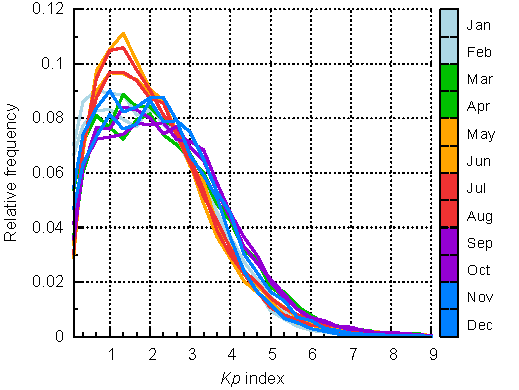
\includegraphics[width=0.46\textwidth]{figures_of_mine/chapter2/Kp_histogram_monthly.pdf}
		}{
			\caption[\lofimage{figures_of_mine/chapter2/Kp_histogram_monthly.pdf}I created the figure myself.]
			{Average monthly \Kp{} frequency distributions of the time period 1932--2016, colored by month of the year. The \Kp{} data is obtained from the GFZ~Potsdam.}
			\label{fig:Kp_histogram_monthly}
		}
		\ffigbox{
			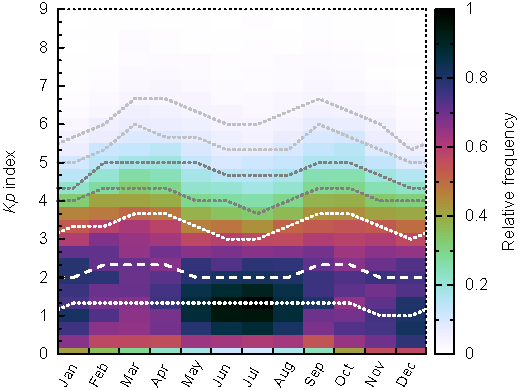
\includegraphics[width=0.46\textwidth]{figures_of_mine/chapter2/Kp_seasonal_e.pdf}
		}{
			\caption[\lofimage{figures_of_mine/chapter2/Kp_seasonal_e.pdf}I created the figure myself.]
			{\Kp{} frequency distributions by month for the time period 1932--2016 with median (white dashed) and quartile isolines (white dotted). The other dotted isolines mark the upper eighth, 16th, 32nd, and 64th parts. The bin size is 1~month and \SI{1/3}{\Kp}~unit respectively.}
			\label{fig:Kp_seasonal_e}
		}
	\end{floatrow}
\end{figure}
These \Kp{} changes arise from seasonal variations of the solar wind parameters at Earth, which stem from Earth's yearly changes in orbital distance and heliographic latitude. The Earth's rotation axis tilt adds another seasonal effect, as the tilt changes the direction of the Earth's magnetic dipole axis to the Sun during the year.

Earth's distance to the Sun varies over the course of a year by \SI{+-1.67}{\percent}, see Appendix~\ref{sec:sun_earth_orbit_geometry}. The solar wind parameters scale via power-law dependencies with solar distance, as it is described in \autoref{chap:empirical_solar_wind_model_for_the_inner_heliosphere} and accordingly in \citet{Venzmer2018}. For example, the solar wind proton density scales with a solar distance exponent of about $-2$, this leads to a yearly variation in density of about \SI{6.7}{\percent}. These yearly variations of the solar wind have direct influence on the \Kp{}~index.

The solar wind influence on the \Kp{}~index depends on its coupling efficiency with the magnetosphere. The rate of magnetic reconnection between solar wind and the Earth's magnetosphere depends on both fields' orientation to each other (parallel/antiparallel). The Sun's rotation axis tilt angle to the ecliptic is \SI{+-7.25}{\degree} and that for Earth is \SI{+-23.44}{\degree}, see also Appendix~\ref{sec:sun_earth_orbit_geometry}. First, the solar wind type composition varies with heliographic latitude, which has consequences for the average values of parameters, such as magnetic field strength and velocity. Second, the tilt of the magnetic dipole axis to the rotation axis -- only a few degrees for the Sun during cycle minima and extreme during solar maxima; and around \SI{10}{\degree} for the Earth -- complicates this system even more.
%geomagnetic dipole tilt: Planetary fact sheet: 11.2 (Model GSFC-12/83)
%variation range in the time period 1930--2016: 9.6--11.5° (http://wdc.kugi.kyoto-u.ac.jp/poles/polesexp.html)

So the \Kp{} variation effects originate from the seasonal change in the solar tilt, the Earth's tilt, and the Earth's solar distance. Thorough analyses of the seasonal variations were already early performed by \citet{Cortie1912} and many others thereafter. Thus, I just assess the bulk magnitude of these effects in order to consider them as relative uncertainties for the solar activity relation (\ref{eq:kp_ssn_relation}). Looking at the \Kp{} frequency distributions by month -- seen in \autoref{fig:Kp_seasonal_e} -- it is apparent that for values ($\Kp{} > 2$), there exist yearly frequency maxima at the equinoxes and frequency minima at the solstices, as was early described by \citet{Cortie1912}. It is evident from the plotted quantiles that this semiannual variation amounts to $1/3$~\Kp~unit for the median \Kp{} and goes up to 4/3~\Kp~units for the rare higher \Kp~values.


\section{Relation between solar wind electric field and \Kp~index}
\label{sec:relation_between_sw_efield_and_kp}
The coupling between the solar wind and the magnetosphere is governed by reconnection and compression of the magnetic field lines, as described in \autoref{sec:solar_wind_coupling_mechanisms}. There exist quite a few coupling functions that are intended to approximate thease processes in relating solar wind quantities with geomagnetic activity (\autoref{sec:coupling_functions}). In this section I settle and work with the solar wind electric field as the coupling function for the purpose of nowcasting the \Kp~index.

The solar wind electric field $\vect{E}$ approximates the rate of magnetic flux aligned with the z"~direction of the GSM coordinates. The electric field y"~component $E_\text{y}$ approximates $\vect{E}$ under special circumstances, see the derivation in \autoref{sec:electric_field_at_the_magnetopause}. $E_\text{y}$ is the product of the radial proton velocity $v_\text{x}$ and the magnetic field z"~component $B_\text{z}$:
\begin{align}
	E_\text{y} = -v_\text{x} \cdot B_\text{z}\,.
\end{align}
In the following analysis, the negative electric field proxy \vBz{} is applied instead, where the vector component $v_\text{x}$ is approximated by the absolute flow speed $v$.

% The solar wind velocity sticks mostly to its radial flow direction, that is, it rarely deviates up to \SI{0.0}{\degree} (correct and cite...).

% argue for \vBz{}\\
% $vB_\text{s}$, large northward fields still contribute to geomagnetic activity.\\
% $vB_\text{T}$, with BT being the field magnitude in the yz"~plane \citep{Newell2007}.\\
% 3hmin(\vBz) performs in correlation slightly better than the sophisticated Newell formula. really?\\


\subsection{Data correlation}
\label{sec:data_correlation}
\Kp{} is defined for 3"~hour time intervals and it represents the maximal variation within this period (see \autoref{sec:kp_index}). Any solar wind parameter that is to be correlated with \Kp{} also should have the same time resolution.

However, in addition to adapting the time resolution, it has to be considered by which means this should be done. Most IMF variations are on shorter time scales than 3~hours. Averaging the IMF over these intervals suppresses features that are important drivers of geomagnetic activity \citep{Savani2017}. Thus, the solar wind parameter's 3"~hourly extreme values are expected to have a stronger correlation with \Kp{} than the 3"~hourly averages.
Commonly the \Kp~index is correlated with 3"~hour or 1"~hour solar wind averages \citep[e.g., ][]{Newell2007,Elliott2013,Savani2017}.

To be able to correlate \Kp{} with solar wind data in a proper way, high resolution solar wind data, that is, much shorter than the 3"~hour resolution, are needed to determine the extrema within each 3"~hour interval.
The \Kp{} time series started in 1932 when there existed no spacecraft to measure solar wind in~situ. Thus, the maximal surveyed time range is restricted by the available in-situ solar wind data.
The OMNI data collection constitutes the longest continuous solar wind measurements made at \SI{1}{\au}. There exist two OMNI data sets with different time resolution -- the hourly version extends back to 1963 and the minutely version extends back to 1981. Although it is shorter, I choose to apply the minutely data, in order to benefit from the higher correlation as discussed below. Thus, the work presented in this chapter is based on the minutely OMNI data set with a time duration of 36~years, spanning from 1981 until end of 2016.

The product \vBz{} is formed and the minutely solar wind data is reduced to 3"~hourly values in two ways: by calculating the averages and the minima.
The reduction to 3"~hour minimum values shifts the \vBz{} frequency distribution asymmetrically to negative values, whereas the averaged data is scattered around zero, see \autoref{fig:histogram_VBzgsm}.
\begin{figure}[htb]
	\begin{floatrow}
		\ffigbox{
			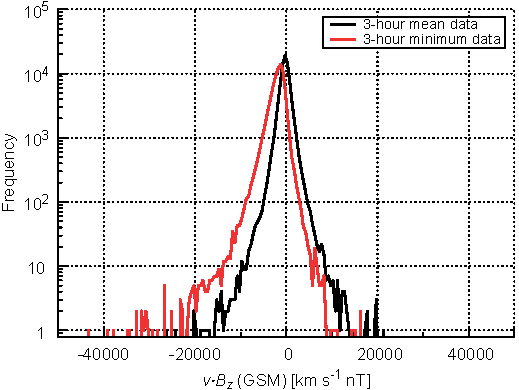
\includegraphics[width=0.46\textwidth]{figures_of_mine/chapter2/histogram_VBzgsm.pdf}
		}{
			\caption[\lofimage{figures_of_mine/chapter2/histogram_VBzgsm.pdf}I created the figure myself.]
			{Frequency distributions for the \vBz{} product. The minutely OMNI data from 1981--2016 is reduced to 3"~hour averages (black line) and 3"~hour minima (red line).}
			\label{fig:histogram_VBzgsm}
		}
%vBz frequency shifts:
% min shift: -1250
% mean shift: -250
% max shift: -750
		\ffigbox{
			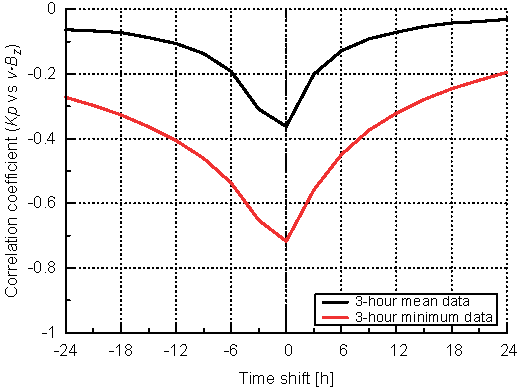
\includegraphics[width=0.46\textwidth]{figures_of_mine/chapter2/cc_lag_data_d_KpvsVBzgsm.pdf}
		}{
			\caption[\lofimage{figures_of_mine/chapter2/cc_lag_data_d_KpvsVBzgsm.pdf}I created the figure myself.]
			{\Kp--\vBz{} correlation coefficients for different time shifts up to \num{+-24}~hours. The minutely OMNI data from 1981--2016 is reduced to 3"~hour averages (black line) and 3"~hour minima (red line).}
			\label{fig:cc_lag_data_d_KpvsVBzgsm}
		}
%highest correlation coefficients:
%min:	0.00000    -0.717240
%mean:	0.00000    -0.362237
%max:	0.00000     0.293137
	\end{floatrow}
\end{figure}

The data is reduced to 3"~hourly values in order to match the \Kp{} data resolution. Both its averages and minima are used to evaluate the advantage of high resolution data by correlating them to the \Kp~index. The \Kp{}--\vBz{} Pearson correlation coefficients for the two differently processed data versions are plotted over time shift in \autoref{fig:cc_lag_data_d_KpvsVBzgsm}. The data with 3"~hour minimum processing shows a much better correlation than the 3"~hour average data. Both curves show a negative correlation and their minima lie at a time shift of zero, which is expected as the OMNI data represents the solar wind at the location of the magnetospheric bow shock. It takes the plasma only a couple of minutes to arrive at the magnetopause and influence the geomagnetic field, for example a study about the Dungey convection cycle by \citet{Zhang2015} accounts for this duration by lagging the OMNI data generally by 5~minutes. I estimate its influence for this analysis to be negligible and thus do not apply such a time shift.

The correlation coefficient for the minimum data reaches a value of $r_\text{min} = -0.72$ and is twice as high as that of the average data $r_\text{avg} = -0.36$.

% Compared with the $vB_\text{s}$ value of $-0.642$ and $vB_\text{T}$ value of $0.551$ from \citet{Newell2007}...\\
% they correlate a 6"~hour solar wind interval to \Kp{} and weight each hour individually.\\


\subsection{Functional dependency for solar wind electric field}
An empirical relation between \vBz{} and \Kp{} is sought by processing the data distribution and fitting an appropriate function to it.
%distribution
The frequency distribution in \Kp--\vBz{} space is shaped like a candle flame, inclined to negative values by a light breeze, see top panel in \autoref{fig:Kp_2dhistogram_VBzgsm_sws_e}. The negative correlation is already apparent.
\begin{figure}
	\fcapside[\FBwidth]{
		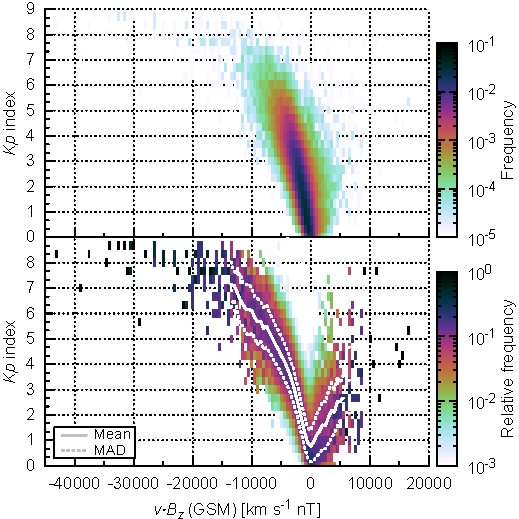
\includegraphics[width=0.6\textwidth]{figures_of_mine/chapter2/Kp_2dhistogram_VBzgsm_sws_e.pdf}
	}{
		\caption[\lofimage{figures_of_mine/chapter2/Kp_2dhistogram_VBzgsm_sws_e.pdf}I created the figure myself.]
		{\Kp{} versus \vBz{} frequency distribution (top panel) and its relative distribution (bottom panel) with the mean \Kp{} values (solid line) and their mean absolute deviation (dotted lines). It is 3"~hour minimum data from the minutely OMNI data set (1981--2016). The bin size is \SI{500}{\km\per\s\nano\tesla} and \SI{1/3}{\Kp}~unit respectively.}
		\label{fig:Kp_2dhistogram_VBzgsm_sws_e}
	}
\end{figure}
%dependency
In order to determine a functional dependency, I focus on the relative frequencies per \vBz-interval and their average \Kp{} values, which are plotted in the bottom panel of \autoref{fig:Kp_2dhistogram_VBzgsm_sws_e}. This probability distribution is asymmetrically V"~shaped around zero, having a larger and steeper negative arm than positive arm. The mean absolute deviation (MAD) from the average \Kp{} value has a mean size of \SI{0.7}{\Kp}~units.
%MAD: 2.211/3 = 0.737 Kp units

The asymmetry also exists for 3"~hour mean data (which is not plotted), thus this effect is not a result of the data reducing method to 3"~hour minima. Rather the steeper negative arm is a consequence of the asymmetric coupling of the solar wind magnetic field direction to the magnetopause, as described in detail in \autoref{sec:solar_wind_coupling_mechanisms}.

%determine fitting functions
For the empirical fit an appropriate type of function has to be constructed. Since the \Kp~index has a quasi-logarithmic scaling (see \autoref{sec:kp_index}), a logarithmic function is the obvious choice as a fit function. Furthermore, the depending argument consists of a product of two solar wind parameters which individually scale logarithmically with \Kp{}. These reasons are why I use the logarithm of a parabola for the fitting approach:
\begin{align}
	f(x) &= \ln\left(x^2\right)	\,.	\label{eq:log_square_function}
\end{align}
I also introduce a horizontal shifting parameter $x'$ because the distribution's center is slightly offset. To be able to replicate the asymmetry in both arms, I further split the fit function at the minimum ($x + x'$) into arms of negative and positive slope:
\begin{align}
	f(x) &=
	\begin{cases}
		\,f_-(x) &\text{for } x + x' < 0	\,,\\
		\,f_+(x) &\text{for } x + x' \ge 0	\,.
	\end{cases}	\label{eq:log_square_fit_function}
\end{align}
This way, both arms can be scaled individually with scaling factors for the negative and positive parts $a_-$ and $a_+$. The resulting logarithmic fit function parts are
\begin{align}
	f_-(x) &= a_- \cdot \ln\left(\left(x + x'\right)^2 + b\right) + y'	\,,\\
	f_+(x) &= a_+ \cdot \left(f_-(x) - f_-\left(-x'\right)\right) + f_-\left(-x'\right)	\,,
\end{align}
with the vertical shifting parameter $y'$ and the depth parameter $b$. The resulting values of the fit coefficients are \mbox{$a_- = 1.258(19)$}, $x' = 163(20)$, $b = \num{1.416(68)e6}$, $y' = -17.04(33)$, and \mbox{$a_+ = 0.467(20)$} for units of [\si{\km\per\s \nano\tesla}].
%high precision values:
% a_- = 1.25788(0.019)\\
% y' = -17.0394(0.33)\\
% a_+ = 0.467039(0.0197)\\
% b = 1.41639e6(0.067795e6)\\
% x' = 162.907(20.642)\\
Thus, the solar wind dependency relation 'condenses' to:
\begin{align}
	\text{\Kp}_-\left(vB_\text{z}\right) &= 1.258 \cdot \ln\left(\left(vB_\text{z} + 163\right)^2 + \num{1.416e6}\right) - 17.04	\,,	\label{eq:kpvsvbz_dependency_function_negative}\\
	\text{\Kp}_+\left(vB_\text{z}\right) &= 0.467 \cdot \left(\text{\Kp}_-\left(vB_\text{z}\right) - \text{\Kp}_-(-163)\right) + \text{\Kp}_-(-163)	\,.	\label{eq:kpvsvbz_dependency_function_positive}
\end{align}
The fit curve is plotted in \autoref{fig:Kp_2dhistogram_VBzgsm_sws_fit_e}.
\begin{figure}
	\fcapside[\FBwidth]{
		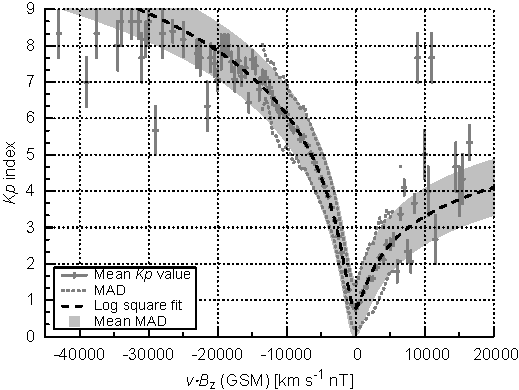
\includegraphics[width=0.6\textwidth]{figures_of_mine/chapter2/Kp_2dhistogram_VBzgsm_sws_fit_e.pdf}
	}{
		\caption[\lofimage{figures_of_mine/chapter2/Kp_2dhistogram_VBzgsm_sws_fit_e.pdf}I created the figure myself.]
		{Mean \Kp{} values (+) and MAD values (dotted lines) per \vBz~interval. The error bars represent the relative data count. The logarithmic fit (dashed line) is plotted with a mean MAD band (shaded area). The splitted function (\ref{eq:log_square_fit_function}) is used for the weighted fit.}
		\label{fig:Kp_2dhistogram_VBzgsm_sws_fit_e}
	}
\end{figure}
The error bars of the data points indicate the relative data count per \vBz{} interval. Those points which deviate far from the fit curve (e.g., below the left arm and above the right arm) stem from single 3"~hour periods. A look into the data revealed that all data outside the range \SIrange{-14000}{8000}{\km\per\s\nano\tesla} is related to CMEs. Thus, the deviating points are caused by individual CME events, for example, the two points with a \Kp{} of $8-$ near \SI{10000}{\km\per\s\nano\tesla} belong to two CMEs\footnote{For reference: the 3"~hour intervals began at 2000-07-16~00:00 and 2005-05-15~09:00} with in-situ velocities of about \SI{1000}{\km\per\s} and a positive $B_\text{z}$ of the order \SI{30}{\nano\tesla}.

% warning lead time
This derived E"~field relation can well be applied with the solar wind real-time measurements that are continuously being made by spacecraft located at L1. However, the heads-up time for warnings from this location is relatively short having only a few tens of minutes, whereas remote observations via solar imagers and coronagraphs allow for longer lead times of a few days. In principle, the E"~field relation could also be applied to remote forecast situations, however, IMF strength and orientation are not yet properly predictable from current prediction methods that rely on remote observations.


\section{Relations between CME/stream velocities and \Kp~index}
\label{sec:relations_between_cme_stream_v_and_kp}
In order to still benefit from the enhanced warning lead times obtained from remote observations, the solar wind velocity has to be employed. It is the only parameter left which is to a certain degree reliably forecastable from remote observations. In fact, solar wind velocity and \Kp~index correlate quite well -- \citet{Machol2013} even proposed a linear function of the \Kp~index as a best proxy for corrupted real-time velocity measurements made by the ACE spacecraft. For one, the velocity can even be used for persistence forecast, as it has the highest autocorrelation time of all major solar wind parameters -- with \SI{59}{\hour} it is much higher than that with the lowest autocorrelation time of \SI{4}{\hour}, which is indeed the $B_\text{z}$~GSM component \citep{Elliott2013}.
It is clear that the strength of the southward IMF component is the most dominant solar wind parameter for the driving of geomagnetic activity. The velocity shows a strong correlation during CME conditions as well, however, infact during high speed streams (HSSs) the velocity is considered the most dominant parameter for driving the geomagnetic activity \citep{Holappa2014}.

% separating CMEs and streams
In order to forecast the \Kp~index from remotely derived velocity values, it makes sense to analyze CMEs and solar wind streams separately. The distinct generation mechanisms of CMEs and solar wind streams show in their different appearance: CMEs are event-like and streams are of continuous nature. Therefore these two solar wind structures require completely different forecast methods (\autoref{sec:solar_wind_nowcast_and_forecast_to_earth}).
In the following, I use an existing list of solar wind structures to separate between CME and solar wind stream data, calculate 3"~hour velocity values, and correlate them with the \Kp~index. Functional dependencies are derived for obtaining \Kp{} proxies from both structure types separately.

\subsection{Solar Wind Structures list}
For the separation of CME and stream data, I use the list of Solar Wind Structures (SWS) created and updated by \citet{Richardson2000} and \citet{Richardson2012}. They characterized the near-Earth solar wind into periods related to slow wind, fast wind, and CMEs. Their list extends back to 1963 and is mostly based on 1"~hour averages of solar wind parameters from the OMNI data set. However, in the cases where there are gaps in the in-situ data, they consider other indicators for identifying solar wind structures. They achieve a fairly complete classification with the inclusion of data from geomagnetic activity, energetic particles, and cosmic rays.
Their work identifies solar wind structures and flags the time series into four categories: CME-associated flows, slow solar wind, fast solar wind, and undetermined intervals. Periods related to CMEs are defined to also comprise the associated ambient solar wind plasma, which consists of upstream shocks and compressed material. The criterion for differentiating between slow and fast solar wind is a velocity threshold of \SI{400}{\km\per\s}.

The SWS list is made available via registration at CEDARweb\footnote{SWS list at CEDARweb: \urlfoot{http://cedarweb.vsp.ucar.edu/wiki/index.php/Tools_and_Models:Solar_Wind_Structures}}. The updated SWS list (until the end of 2016) was kindly provided by Ian~Richardson.
%List of near-Earth ICMEs since January 1996 by \citet{Cane2003,Richardson2010}. Available as ACE Level~3 data for the period 1995--mid2016\footnote{ACE Level~3 data website -- list of near-Earth ICMEs: \urlfoot{http://www.srl.caltech.edu/ACE/ASC/DATA/level3/icmetable2.htm}}.\\
According to the SWS list, the CME fraction during the 36-year time period considered in the present study, 1981--2016, is \SI{15.4}{\%}, which accumulates to 5.53~years. %and that for the period 1963--2016 is \SI{16.9}{\%} (9.01~years).\\
This percentage is an average value, as the actual short-term fraction varies heavily with the solar activity cycle and with the appearance of individual active regions on the solar surface.

The SWS definition of CME-associated flows makes sense for the present study as the causes of the strongest geomagnetic storms are both the compression of the magnetic field within the shock fronts of fast CMEs and the enhanced field strength of the driving magnetic clouds \citep{Bothmer1995}. In the following part of this study, I refer to the combination of the SWS categories slow and fast solar wind simply as solar wind streams. These periods are composed entirely from a mixture of slow wind flows, fast wind streams, and their interaction regions.

\subsection{Data correlation}
Again, as done before for the data processing of the E"~field analysis, 3"~hour average as well as extreme velocities are calculated using the minutely OMNI data in order to test for a higher correlation with \Kp{}. The comparison between the 3"~hour average and the 3"~hour maximum frequency distributions shows that their mean positions are shifted slightly, having velocities of \SI{405}{\km\per\s} and \SI{425}{\km\per\s} respectively (\autoref{fig:histogram_V_d}).
%the SWS1 mean raises from 435 to 455~km/s in 3hmax data...\\
\begin{figure}[htb]
	\begin{floatrow}
		\ffigbox{
			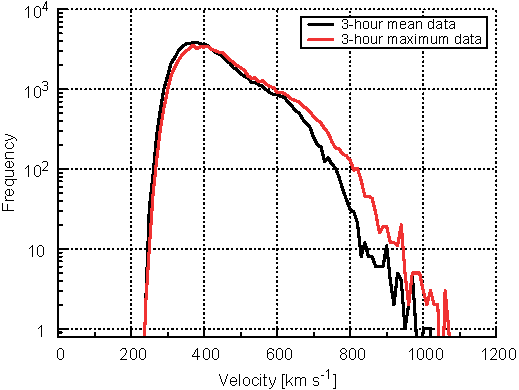
\includegraphics[width=0.5\Xhsize]{figures_of_mine/chapter2/histogram_V_d.pdf}
		}{
			\caption[\lofimage{figures_of_mine/chapter2/histogram_V_d.pdf}I created the figure myself.]
			{Solar wind velocity frequency distributions for the 3"~hour average and 3"~hour maximum data. The minutely OMNI data from the period 1981--2016 is used.}
			\label{fig:histogram_V_d}
		}
		\ffigbox{
			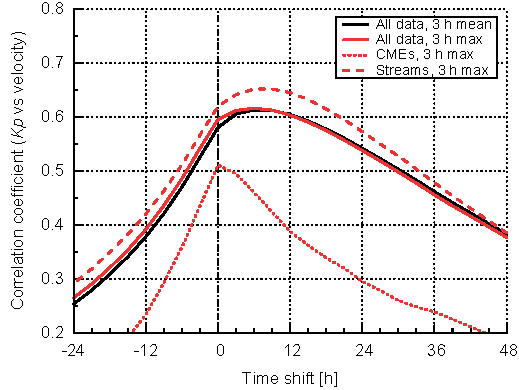
\includegraphics[width=\Xhsize]{figures_of_mine/chapter2/cc_lag_sws_f.pdf}
		}{
			\caption[\lofimage{figures_of_mine/chapter2/cc_lag_sws_f.pdf}I created the figure myself.]
			{\Kp{}--velocity correlation coefficients for time shifts in the range from $-24$ to 48~hours. The correlations are plotted for the whole solar wind data (solid lines), for solar wind streams without CMEs (dashed line), and for CMEs only (dotted line). The data used is the 3"~hour averages (black) and the 3"~hour maxima (red) of the minutely high resolution OMNI data from the period 1981--2016.}
			\label{fig:cc_lag_sws_f}
		}
	\end{floatrow}
\end{figure}

The \Kp{} correlations with the average and maximum processed data show that both are nearly identical, see \autoref{fig:cc_lag_sws_f}. Their maxima lie at a time shift of 6"~hours with correlation coefficients of 0.61 and 0.62 respectively, see \autoref{tab:correlation_coefficients_kpvsv}.
\begin{table}
	\caption{The highest correlation coefficients and their time lags of the \Kp{}--velocity relations for the different data versions: 3"~hour averaged data, 3"~hour maximum of all data, CME, and stream data. The values are based on the minutely high resolution OMNI data from the time period 1981--2016.}
	\label{tab:correlation_coefficients_kpvsv}
	\centering
	\begin{tabular}{lccc}
		\hline\hline
		Data	&3"~hour processing	&Time lag [hours]	&Correlation coefficient\\
		\hline
		All data	&averages	&6	&0.613\\
		All data	&maxima	&6	&0.622\\
		CMEs	&maxima	&0	&0.511\\
		Streams	&maxima	&9	&0.661\\
		\hline
	\end{tabular}
\end{table}
% the best lag times are:\\
% sws: +6 h\\
% sws1: 0 h\\
% sws23: +9 h\\
% 
% correlation coefficients\\
% SWS1\\
% 0	0.511093\\
% SWS23\\
% lag	cross	auto x	auto y\\
% -3	0.660694\\
% 0	0.620113\\
% SWS\\
% lag	cross	auto x	auto y\\
% -2	0.621539\\
% 0	0.595784\\

The CME and stream parts of the 3"~hour maximum data are examined separately by filtering the corresponding periods using the SWS list. Both parts are correlated independently with the \Kp~index. The correlations for CME related data are lower than that for all solar wind. Their maximal correlation coefficient has a value of 0.51 and is without time shift.
Solar wind streams show higher correlations with \Kp{} and the correlation's maximum value 0.66 has a positive time shift of 9~hours, which means that the \Kp~index forecasts the velocity of solar wind streams 9~hours in advance.
This positive time shift may be explained from the occurence of interaction regions followed by HSSs. When a slow solar wind stream is followed by a fast one, the compression at their interface leads to enhanced solar wind densities and magnetic field strengths. The peak velocity of a HSS naturally appears after the interaction region. Therefore the \Kp-impact from the enhanced magnetic field might be correlated with the higher velocity of the trailing HSS, resulting in the observed positive time shift.

The broader correlation curve for streams (\autoref{fig:cc_lag_sws_f}) seems to be owed to their continuous nature, whereas the more peaked CME curve can be a result of their event-like nature. The significantly higher correlation coefficient seen for streams might replicate the velocity's dominating role for geomagnetic activity during HSSs \citep{Holappa2014}.

For \vBz{} the correlations with \Kp{} are very different for 3"~hour averages and extrema, at the same time the same procedure with velocity results in two almost identical correlations. I suggest this situation can be explained by the very different autocorrelation times of $B_\text{z}$ and velocity \citep{Elliott2013}.

% Compare with Newell's $r_v = 0.582$.\\

\subsection{Functional dependencies for CME and stream velocities}
The general \Kp--velocity dependency in the solar wind is apparent from the tilt of its distribution, see top panel of \autoref{fig:Kp_2dhistogram_V_sws_d}.
\begin{figure}
	\fcapside[\FBwidth]{
		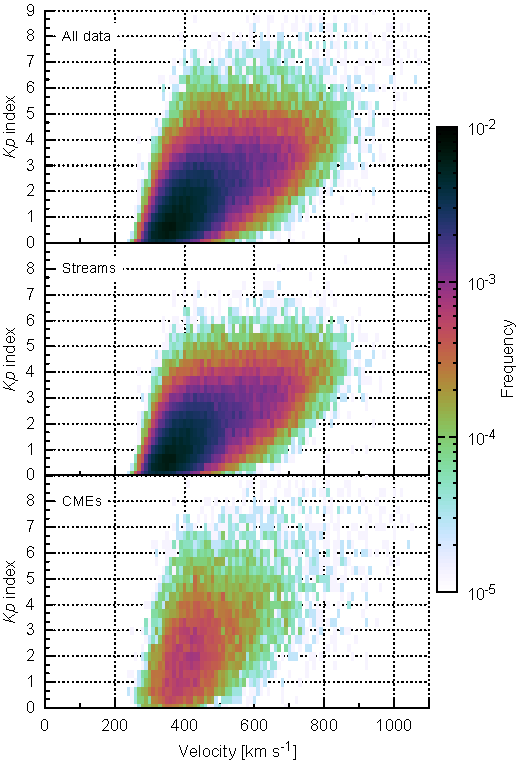
\includegraphics[width=0.6\textwidth]{figures_of_mine/chapter2/Kp_2dhistogram_V_sws_d.pdf}
	}{
		\caption[\lofimage{figures_of_mine/chapter2/Kp_2dhistogram_V_sws_d.pdf}I created the figure myself.]
		{\Kp--velocity distributions for all solar wind data, for solar wind streams, and for CMEs. The data used is the 3"~hour maximum of the minutely high resolution OMNI data from the time period 1981--2016. The SWS list from \citet{Richardson2012} is used for the separation between CME and stream data. The bin size is \SI{10}{\km\per\s} and \SI{1/3}{\Kp}~unit respectively.}
		\label{fig:Kp_2dhistogram_V_sws_d}
	}
\end{figure}
The distribution is inclined to positive values but very broad, that is, in the typical solar wind velocity range it spans over more than half of the total \Kp{} range. The comparison with the filtered data shows that \Kp{} values \num{>6} and velocities \SI{>850}{\km\per\s} are almost always associated with CME related periods, see middle and bottom panel of \autoref{fig:Kp_2dhistogram_V_sws_d}.

% Functional dependency for CME velocity
In order to determine a functional relation between \Kp{} and CME velocity, I look at the relative \Kp{} frequencies for each \SI{10}{\km\per\s} velocity interval. The relative frequencies are plotted in the bottom panel of \autoref{fig:Kp_2dhistogram_V_sws1_c2}.
\begin{figure}
	\fcapside[\FBwidth]{
		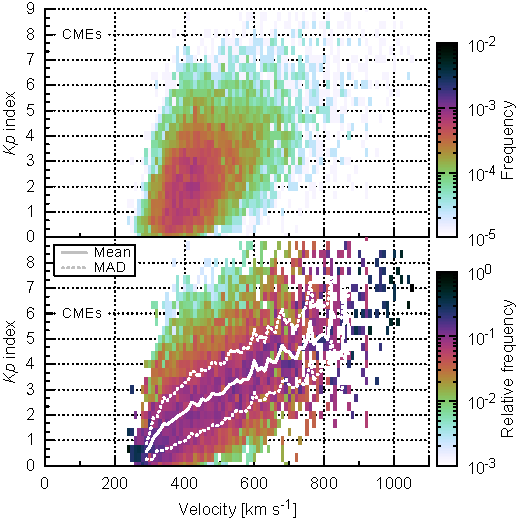
\includegraphics[width=0.6\textwidth]{figures_of_mine/chapter2/Kp_2dhistogram_V_sws1_c2.pdf}
	}{
		\caption[\lofimage{figures_of_mine/chapter2/Kp_2dhistogram_V_sws1_c2.pdf}I created the figure myself.]
		{CME part of the \Kp--velocity distribution (same as third panel of \autoref{fig:Kp_2dhistogram_V_sws_d}) and its relative distribution per velocity interval with the mean \Kp{} values (solid line) and their MAD (dotted lines). The bin size is \SI{10}{\km\per\s} and \SI{1/3}{\Kp}~unit respectively.}
		\label{fig:Kp_2dhistogram_V_sws1_c2}
	}
\end{figure}
The average \Kp{} value seems to scale almost linear with the solar wind velocity. The MAD of the average \Kp{} value has a mean size of about \SI{1.1}{\Kp~units}.
%MAD: 3.338/3 = 1.113 Kp units
%determine fitting function
Again, as the \Kp~index has a quasi-logarithmic scaling, a logarithmic function is the obvious choice for the fitting process. Thus, the logarithmic function
\begin{align}
	f(x) = a \cdot \ln\left(x + x'\right) + y'	\label{eq:log_offset_fit_function}
\end{align}
is used for the fit, with the scaling factor $a$, the location parameter $x'$, and the vertical shifting parameter $y'$. The resulting fit parameters are $a = \num{10.6(34)}$, $x' = \num{8.1(43)e2}$, and $y' = \num{-73(28)}$, with the velocity in units of [\si{\km\per\s}].
%10.6075 (3.4)\\
%-73.1694 (28.)\\
%806.943 (430)\\
They lead to the CME dependency function
\begin{align}
	\text{\Kp}_\text{CME}(v) = 10.6 \cdot \ln(v + 810) - 73	\,,	\label{eq:kpvsv_CME_dependency_function}
\end{align}
which is plotted in \autoref{fig:Kp_2dhistogram_V_sws1_fit_e}.
\begin{figure}
	\fcapside[\FBwidth]{
		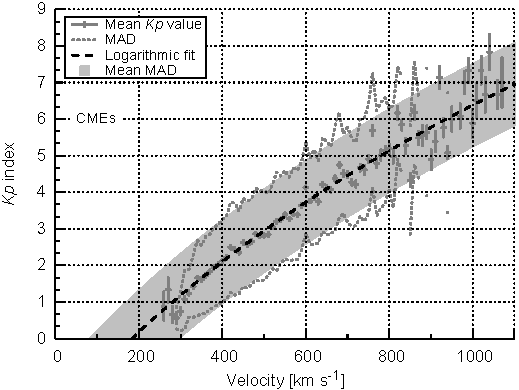
\includegraphics[width=0.6\textwidth]{figures_of_mine/chapter2/Kp_2dhistogram_V_sws1_fit_e.pdf}
	}{
		\caption[\lofimage{figures_of_mine/chapter2/Kp_2dhistogram_V_sws1_fit_e.pdf}I created the figure myself.]
		{Mean \Kp{} values (+) and MAD values (dotted lines) per velocity interval for the CME part of the data. The error bars represent the relative data count. The logarithmic fit (dashed line) is plotted with a mean MAD band (shaded area). The function (\ref{eq:log_offset_fit_function}) is used for the weighted fit.}
		\label{fig:Kp_2dhistogram_V_sws1_fit_e}
	}
\end{figure}
This empirical relation can be used to forecast the \Kp{}~index from a predicted CME arrival velocity, e.g., obtained from analyses of remote coronagraph observations.

% Functional dependency for stream velocity
The procedure for the functional dependency on stream velocity is the same as that for the CME velocity. However, in the case of solar wind stream velocities, the correlation coefficient is higher when the data is shifted by 9~hours (\autoref{fig:cc_lag_sws_f}).
I use this shifted data and look at the relative frequencies per velocity interval in order to find a functional dependency between \Kp{} and velocity, see bottom panel of \autoref{fig:Kp_2dhistogram_V_sws23_d}.
\begin{figure}
	\fcapside[\FBwidth]{
		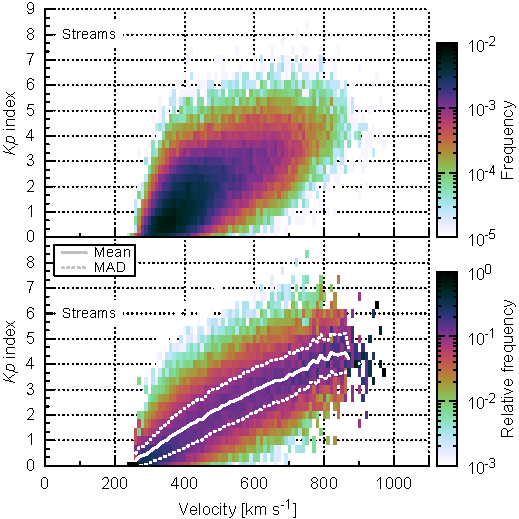
\includegraphics[width=0.6\textwidth]{figures_of_mine/chapter2/Kp_2dhistogram_V_sws23_d.pdf}
	}{
		\caption[\lofimage{figures_of_mine/chapter2/Kp_2dhistogram_V_sws23_d.pdf}I created the figure myself.]
		{Stream part of the \Kp--velocity distribution (similar to second panel of \autoref{fig:Kp_2dhistogram_V_sws_d}, but with the data shifted by 9~hours) and its relative distribution per velocity interval with the mean \Kp{} values (solid line) and their MAD (dotted lines). The bin size is \SI{10}{\km\per\s} and \SI{1/3}{\Kp}~unit respectively.}
		\label{fig:Kp_2dhistogram_V_sws23_d}
	}
\end{figure}
Again, the mean \Kp{} value scales almost linear with the velocity. The distribution is much narrower than that for CMEs -- the MAD from the average \Kp{} has only a mean size of about \SI{0.7}{\Kp}~units.
%MAD: 2.226/3 = 0.742 Kp units
%MAD: 2.332/3 = 0.777 Kp units for 300--900km/s
%MAD: 2.389/3 = 0.796 Kp units for 350--900km/s
%MAD: 2.454/3 = 0.818 Kp units for 350--850km/s

%determine fitting function
Again, I use the logarithmic function (\ref{eq:log_offset_fit_function}) for the fitting process. The resulting values of the fit parameters are \mbox{$a = \num{5.88(38)}$}, $x' = \num{2.99(49)e2}$, and $y' = \num{-3.70(29)e1}$, with the velocity in units of [\si{\km\per\s}].
%a1 = 5.88(38)
%b1 = -37.0(29)
%x1 = 299(49)
This leads to the solar wind stream dependency function
\begin{align}
	\text{\Kp}_\text{Stream}(v) = 5.88 \cdot \ln(v + 299) - 37.0	\,,	\label{eq:kpvsv_stream_dependency_function}
\end{align}
which is plotted in \autoref{fig:Kp_2dhistogram_V_sws23_fit_e}.
\begin{figure}
	\fcapside[\FBwidth]{
		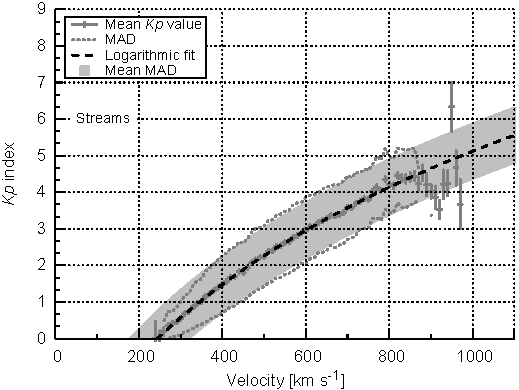
\includegraphics[width=0.6\textwidth]{figures_of_mine/chapter2/Kp_2dhistogram_V_sws23_fit_e.pdf}
	}{
		\caption[\lofimage{figures_of_mine/chapter2/Kp_2dhistogram_V_sws23_fit_e.pdf}I created the figure myself.]
		{Mean \Kp{} values (+) and MAD values (dotted lines) per velocity interval for the stream part of the data, shifted by 9~hours. The error bars represent the relative data count. The logarithmic fit (dashed line) is plotted with a mean MAD band (shaded area). The function (\ref{eq:log_offset_fit_function}) is used for the weighted fit.}
		\label{fig:Kp_2dhistogram_V_sws23_fit_e}
	}
\end{figure}
This empirical relation can be used to forecast the \Kp{}~index from an estimated stream velocity, e.g., obtained from remote coronal hole analyses.

The stream velocity curve is smaller and its slope is less steep than that obtained from the CME velocities. CMEs with a speed of \SI{500}{\km\per\s} cause on average a 2/3~\Kp~unit higher \Kp{} than a stream of the same speed would -- for CMEs with \SI{1000}{\km\per\s} this gap even increases to 4/3~\Kp~units. This difference in \Kp{} magnitude between the two velocity relations is due to the generally larger magnetic field strength in CMEs compared with streams having the same velocity.


\section{Prediction performance}
\label{sec:prediction_performance}
% prediction model performances
The derived empirical relations are chosen for their high correlation coefficients. However, the correlation coefficient itself does not represent the performance of a model as the coefficient depends highly on the scatter of the underlying distribution. Therefore \citet{Wing2005} advise to additionally provide scatterplots and skill scores for the evaluation of predictive models. In the following, I present the forecast errors and determine the true skill statistics as measures for the prediction performance of the drived empirical models.

% persistence
The quality of predictions can be assessed by how they compare to a simple persistence model \citep{Detman1999}. In the case at hand, the persistence consists of the official \Kp{} value from the previous 3"~hour interval. The persistence performance is obtained from the complete \Kp{} time span 1981--2016.

% prediction performance
In order to evaluate all models' prediction performances, their forecast errors are calculated. Forecast errors are the differences between the predicted and the actual values. The resulting performances of the persistence and the three models are displayed together with the corresponding positive and negative standard deviations in \autoref{fig:model_performance_d}.
\begin{figure}
	\fcapside[\FBwidth]{
		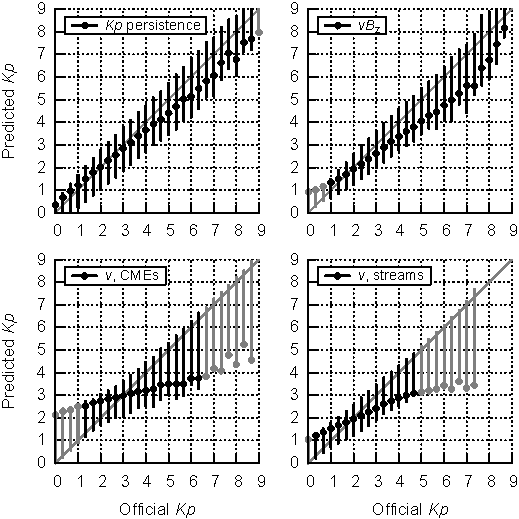
\includegraphics[width=0.6\textwidth]{figures_of_mine/chapter2/model_performance_d.pdf}
	}{
		\caption[\lofimage{figures_of_mine/chapter2/model_performance_d.pdf}I created the figure myself.]
		{Prediction performance of \Kp{} persistence and the three derived empirical \Kp{} relations. The forecast errors are the differences between the predicted and the actual values. They are calculated from the same data and time range as the relations themselves. The errorbars denote one positive and one negative standard deviation. Forecast errors with one-sided deviations are plotted in gray. Perfect predictions are indicated by the diagonal lines.}
		\label{fig:model_performance_d}
	}
\end{figure}
The deviations to the forecast errors can be completely one-sided if the actual \Kp{} values are always being over- or underestimated (in the figure these points are plotted in gray). This happens at the extreme ends of the \Kp{} range -- I denote the range in between as proper range.

The empirically derived solar wind relations do not cover the whole \Kp{} range from 0 to 9 within the distributions of observed values. Only the \Kp{} values with more than one observed data point are considered for deriving the relations' prediction performances. This excludes the \Kp{}~9 values and in case of the velocity relation for streams also the values \Kp{}~7.7 and above.

% persistence performance
The persistence performs fairly well, as its forecast error is less than 0.7~\Kp{} units up to a \Kp{} of 5.7. At and above a \Kp{} of 6 the error is underestimated with a maximum deviation of 1.3~\Kp{} units.
% vBz performance
The derived \vBz{} function (\ref{eq:kpvsvbz_dependency_function_negative} and \ref{eq:kpvsvbz_dependency_function_positive}) does only coincide with significant data in the \Kp{} range 1 to 8.7, in particular because the minimum of the \vBz{} function is larger than 0.7~\Kp{} (\autoref{fig:Kp_2dhistogram_VBzgsm_sws_fit_e}). The model performs reasonably well at and below a \Kp{} of 5 with forecast errors smaller than 1~\Kp~unit. Larger \Kp~values are underestimated and deviate up to 1.7~\Kp~units from the predicted values.
% v CME performance
In the case of the velocity relation for CMEs, the \Kp{} magnitude is overestimated below a \Kp{} of 3 and underestimated above and the proper range lies between 1.3 and 6.3. In the range between a \Kp{} of 1 to 5 the forecast errors are smaller than 1.3~\Kp~units. Above, the error rises up to 4~\Kp~units at a \Kp{} of 8.7.
% v stream performance
For the velocity relation for streams, the proper range goes from 0.3 to 4.3 -- the magnitude is overestimated below a \Kp{} of 2 and underestimated above. The forecast errors are smaller than 1.3~\Kp~units throughout the proper range. Above, the error rises up to 4~\Kp~units at a \Kp{} of 7.3.
% conclusion
The model based on the \vBz{} relation is more accurate than those based purely on the velocity. This is expected, however, the \vBz{} relation is still eclipsed by the persistence model.

% true skill score
In order to further test the derived models for their predictive value, I derive their true skill statistic (TSS) -- a common tool for forecast verification. The TSS is a skill score based on the contingency table that categorizes forecasted and observed events. The score is the difference between the forecast hit rate and the false alarm rate. Its range goes from $-1$ to 1, where 1 indicates an ideal prediction and 0 a random prediction. I give more detailed information about the TSS in the Appendix~\ref{sec:true_skill_statistic}. This method is the prevalent form of forecast verification in \Kp{} models \citep{Detman1999,Wing2005,Savani2017}. It is defined that each single 3"~hour \Kp{} interval represents an event and a hit occurs when both the forecasted and observed \Kp{} exceed a specified threshold. I adopt these criteria to make the results comparable. Therefore the TSS is derived as a function of \Kp{} threshold -- the results for persistence and the three models are plotted in \autoref{fig:true_skill_score}.
\begin{figure}
	\fcapside[\FBwidth]{
		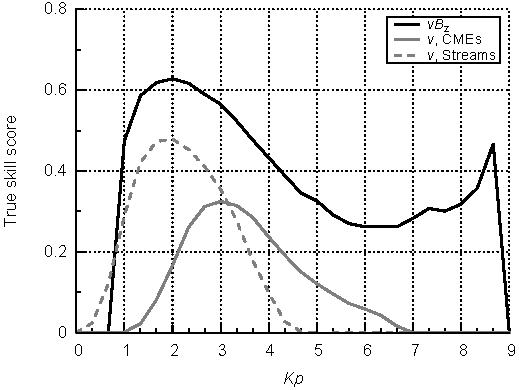
\includegraphics[width=0.6\textwidth]{figures_of_mine/chapter2/true_skill_score.pdf}
	}{
		\caption[\lofimage{figures_of_mine/chapter2/true_skill_score.pdf}I created the figure myself.]
		{True skill scores for the \Kp{} persistence and the three predictive models as a function of \Kp{} threshold. The scores are calculated from the same data and time range as the relations themselves.}
		\label{fig:true_skill_score}
	}
\end{figure}

The E"~field relation reaches its peak at a \Kp{} of 2 with a TSS of 0.63, it then decreases to a local minimum at \Kp{} 6 with a TSS of 0.26. To higher \Kp{} values, the TSS increases again and reaches 0.47 at a \Kp{} of 8.7. This increase is due to the dominant number of correct null forecasts that make the TSS approach the hit rate \citep{Doswell1990} -- it is a bias inherent to the TSS in case of rare event forecasting. Both velocity relations have throughout their \Kp{} ranges a significantly lower TSS. The CME relation shows a peak TSS of 0.32 at a \Kp{} of 3 and the stream relation a peak TSS of 0.48 at a \Kp{} of 2. Thus, the TSS gain from the additional $B_\text{z}$ component is about \numrange{0.15}{0.2}.

The persistence forecast clearly outperforms the other prediction models, especially in the high \Kp{} range. However, as \citet{Detman1999} stated, it has no warning value because it can only predict a high \Kp{} value after a high \Kp{} value was already observed. Thus, the persistence always misses the onset of a geomagnetic storm, whereas solar wind based models can provide at least a nowcast if not actually a short lead time from the distance of the in-situ measurement location at L1.

% statistics summary table
In order to compare the \Kp{} forecast skill metrics with other models, \citet{Savani2017} use a threshold of $\Kp{} \geq 5$. They choose this value because of the geomagnetic storm scale (G"~scale) developed by NOAA's SWPC. The G"~scale relates the \Kp~index to five levels from G1 to G5\footnote{NOAA Space Weather Scales website: \urlfoot{http://www.swpc.noaa.gov/noaa-scales-explanation}}. The starting level G1 translates to a \Kp{} of 5. I stick to this definition and provide a statistics summary of the \Kp{} persistence and the three derived models in \autoref{tab:model_statistics_table}.
\begin{table}[htb]
	\caption{Statistics of the different prediction models. The metrics are calculated for a threshold hit criteria of $\Kp{} \geq 5$ for the same data and time range as the relations themselves.}
	\label{tab:model_statistics_table}
	\centering
	\begin{tabular}{lcccc}
		\hline\hline
		\multirow{2}{*}{Parameter}	&\Kp{} persistence	&E"~field	&CME velocity 	&Stream velocity\\
			&$\Kp(t-1)$	&$\Kp(\text{\vBz})$	&$\Kp(v_\text{CME})$	&$\Kp(v_\text{Streams})$\\
		\hline
		Time shift [hours]	&3	&0	&0	&9\\
		Event count	&\num{105192}	&\num{79276}	&\num{12116}	&\num{65774}\\
		Correlation coefficient	&0.81	&\num{-0.72}	&0.51	&0.66\\
		\hline
		Proportion correct	&0.96	&0.97	&0.88	&0.98\\
		Hit rate	&0.55	&0.33	&0.13	&0\\
		False alarm rate	&0.02	&0	&0.01	&0\\
% 		FAR	&0.45	&0.24	&0.35	&1\\
% 		DFR	&0.02	&0.03	&0.11	&0.02\\
		True skill score	&0.53	&0.33	&0.12	&0\\
		Proper range [\Kp{}]	&\numrange{0.3}{8.7}	&\numrange{1.0}{8.7}	&\numrange{1.3}{6.3}	&\numrange{0.3}{4.3}\\
		\hline
	\end{tabular}
\end{table}

For the stream velocity relation, the defined \Kp{} threshold is of little use as its proper \Kp~range is below the defining geomagnetic storm value of \Kp{}~5. The maximal velocity of solar wind streams is limited by the coronal temperatures \citep{Parker1958} and is observed to be around \SI{900}{\km\per\s}. That is why solar wind plasma associated with streams on average provoke \Kp{} values below 5o, that is, geomagnetic storms  be predicted via the stream relation.

% comparison
The E"~field model has a TSS of 0.33 at a \Kp{} of 5, this can be compared with the Wing APL models \citep[Fig.~13]{Wing2005}. The Wing APL model~3 predicts \Kp{} 1~hour in advance and uses the solar wind parameters velocity, density, magnetic field strength, and $B_\text{z}$ as input sources for a neural network based model. The additionally considered parameters (density and absolute magnetic field strength) boost the corresponding TSS to about 0.7. The Wing APL model~1 incorporates \Kp{} nowcast values in addition to the solar wind parameters and achieves this way a TSS of about 0.8.

The BSS model developed by \citet{Savani2015,Savani2017} predicts the magnetic field in CMEs arriving at Earth and derives their geomagnetic response. For a total of eight CME events the BSS model shows a TSS of 0.34, when investigating only restricted periods of ``active solar wind'' \citep[Tab.~3]{Savani2017}.
% Costello model (neural network, input: sw): about 0.45\\
% Wing APL model 1 (1 h, neural network, input: Kp nowcast + sw): about 0.8\\
% Wing APL model 2 (4 h, neural network, input: Kp nowcast + sw): about 0.7\\
% Wing APL model 3 (1 h, neural network, input: sw): about 0.7\\
% BSS model for eight CME events has $\mathit{TSS} = 0.34$ \citep[Tab.~3]{Savani2017}\\


\section{Discussion}
\label{sec:discussion_ch2}
% solar activity influence
For the solar wind predictive \Kp{} models, the influence of the solar activity is not considered despite its contribution of a variation of about 1.6~\Kp~units (see \autoref{sec:kp_long_term_variations}). A detailed analysis of the solar activity's influence on the \Kp{} prediction behavior lies outside the scope of this thesis. Nevertheless, it would be worth examining the solar cycle's influence on the relations, especially as \citet{Wing2005} note that the predictability of \Kp{} slightly scales with solar activity.
\citet{Gopalswamy2014} indicate in particular that low solar activity leads to a decreased geomagnetic effectiveness of CMEs in general. The reason is the reduced pressure within the heliosphere, which allows for a greater expansion of CMEs, resulting in the dilution of the magnetic field in the CME as well as weaker fields in the accompanying ambient compression regions.
% % low solar activity influence on geomagnetic storms/space weather
% \textit{The weaker solar activity cycle 24 seems to have important consequences for CMEs in the heliosphere: CMEs expand anomalously due to reduced heliospheric pressure leading to the increased observed rate of small CMEs, halos originating far from the disk center, and mild space weather (\citep{Gopalswamy2014}, 2015a; Petrie 2015).\\
% The total pressure in the heliosphere (magnetic + plasma) is reduced by ca. 40\%, which leads to the anomalous expansion of CMEs explaining the increased slope. The excess CME expansion contributes to the diminished effectiveness of CMEs in producing magnetic storms during cycle 24, both because the magnetic content of the CMEs is diluted and also because of the weaker ambient fields \citep{Gopalswamy2014}.\\
% }


% in-situ plots
In the following, I take two sample periods of solar wind in-situ data and apply the predictive \Kp{} models to compare their output qualitatively with the actual measured \Kp~index. First, I discuss a 2"~month period from the maximum of the solar activity cycle~24 and second, I zoom into a 6"~day sub-period containing a CME.

% 5-week sample period
The 2"~month sample period of solar wind and \Kp{} data is displayed in \autoref{fig:example_sw_plot_1month_b_9hshift_2013-5-1_65}.
\begin{figure}[htb]
	\centering
	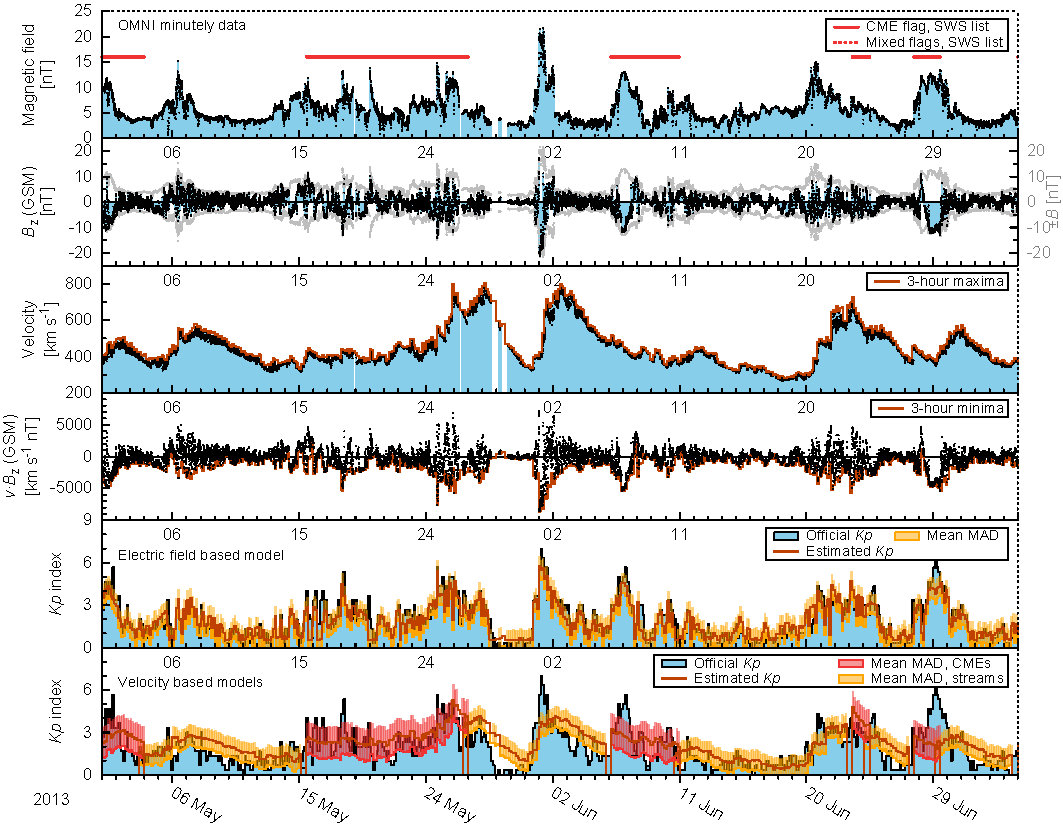
\includegraphics[width=\textwidth]{figures_of_mine/chapter2/example_sw_plot_1month_b_9hshift_2013-5-1_65.pdf}
	\caption[\lofimage{figures_of_mine/chapter2/example_sw_plot_1month_b_9hshift_2013-5-1_65.pdf}I created the figure myself.]
	{Solar wind parameters, official \Kp~index, and estimated \Kp{} indices for the 65"~day time period from 1~May to 5~July 2013. The solar wind parameters are the magnetic field strength, its z"~component in GSM coordinates, the velocity, and the product of the latter two. I also plot the velocity's 3"~hour maxima and the \vBz{}'s 3"~hour minima for illustration. The \Kp{} estimates based on the electric field and the velocity relations are displayed together with their mean MAD bands. The \Kp{} estimates from both velocity relations are chosen according to the periods flagged as CMEs or streams in the SWS list (red lines in top panel). The \Kp{} estimate derived from stream velocity is shifted by 9~hours. The solar wind data are from the minutely OMNI data set and the official \Kp~index is obtained from the GFZ~Potsdam.}
	\label{fig:example_sw_plot_1month_b_9hshift_2013-5-1_65}
\end{figure}
The considered period ranges from 1~May to 5~July 2013, when the solar activity cycle~24 had its maximum. The period contains various types of structures, such as HSSs, CIRs, and CMEs.
% describe plot
The plot shows the solar wind IMF strength, its z"~component, the velocity with its 3"~hour maxima, and the electric field \vBz{} with its 3"~hour minima. The \Kp{} estimate based on the electric field relation is displayed together with the official \Kp~index. The CME and stream velocity relations are displayed together with the official \Kp~index as well, however, both velocity relations are chosen according to the periods flagged as CMEs or streams in the SWS list, that is, either via Equation~(\ref{eq:kpvsv_CME_dependency_function}) or (\ref{eq:kpvsv_stream_dependency_function}). The \Kp{} derived from stream velocity is based on the data shifted by 9~hours.

% interprete plot
It can be seen that in the considered period the \Kp{} estimate based on the E"~field traces the actual \Kp~index pretty well within its mean MAD band, whereas the \Kp{} estimates based on both velocity relations do not coincide that well with the actual \Kp~index. The stream velocity based model overestimates small \Kp{} values, which occur during rarefaction regions of declining velocity, whereas compressed regions are underestimated, such as the interaction region on 1~June 2013. The CME velocity based model underestimates the effect of pronounced MCs, as is seen for the CMEs on 6~June and 27~June 2013.

% Elliott2013
A study that differentiates especially between compression and rarefaction regions is that of \citet{Elliott2013}. They compare three threshold techniques to do so: by sorting for density, dynamic pressure, and velocity slope. The three \Kp--velocity distribution panels in \autoref{fig:Kp_2dhistogram_V_sws_d} look indeed very similar to the Figures~3 and~4 from \citet{Elliott2013}. This is because they sort the \Kp{}--velocity distribution for CMEs and streams, use OMNI data, and the SWS list as well, however, they use a different time resolution, data processing, and time period. More precisely, they use 3"~hour averages of the hourly OMNI data set, modify the CME-associated periods of the SWS list with additional constraints, and use data from the time period 1963--2009.

% 6~day sub-period
The second solar wind plot zooms in on the latter CME -- it covers the 6"~day time period from 26~June to 2~July 2013, see \autoref{fig:example_sw_plot_CME_b_9hshift_2013-6-26_6}.
\begin{figure}[htb]
	\centering
	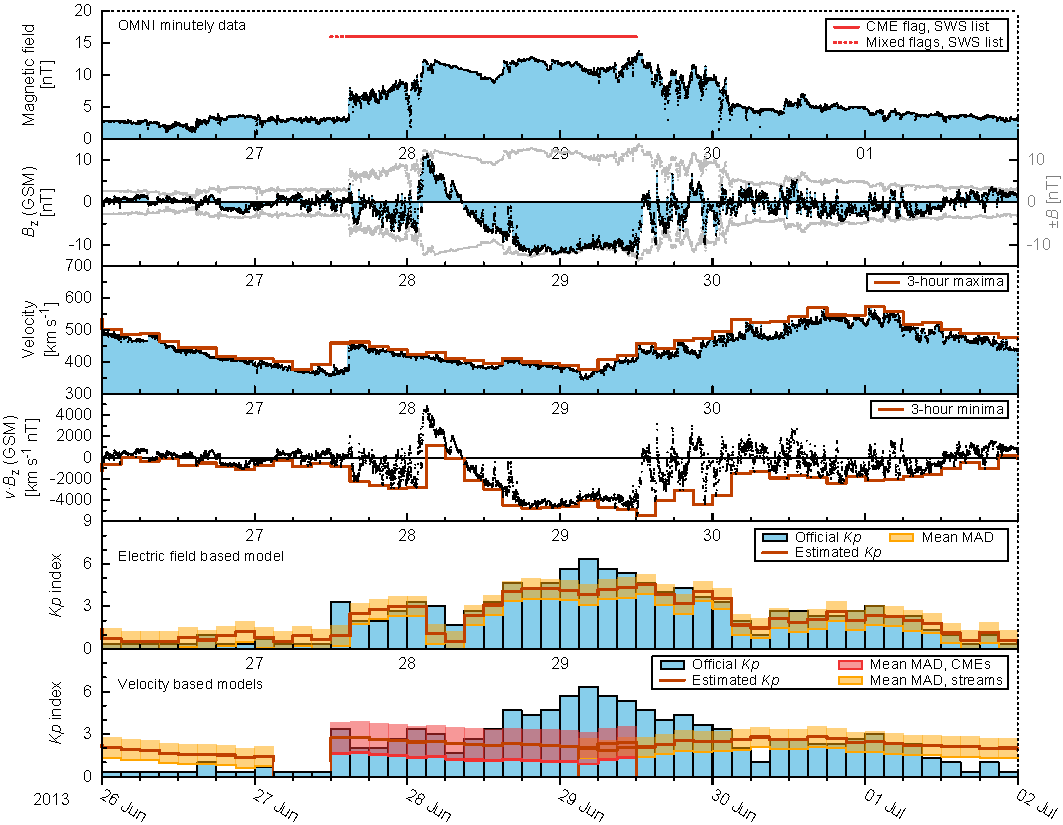
\includegraphics[width=\textwidth]{figures_of_mine/chapter2/example_sw_plot_CME_b_9hshift_2013-6-26_6.pdf}
	\caption[\lofimage{figures_of_mine/chapter2/example_sw_plot_CME_b_9hshift_2013-6-26_6.pdf}I created the figure myself.]
	{Solar wind parameters, official \Kp~index, and estimated \Kp{} indices for the 6"~day time period from 26~June to 2~July 2013. All panels show the same parameters as in \autoref{fig:example_sw_plot_1month_b_9hshift_2013-5-1_65}. The period covers the CME from 27~June 2013, which induced a peak \Kp{} of $6+$.}
	\label{fig:example_sw_plot_CME_b_9hshift_2013-6-26_6}
\end{figure}
The plot shows the same parameters as in the previous plot. This more detailed sample period agrees with the observations made from the previous 2"~month period. In addition, it can be seen that deviations in the \vBz{} based \Kp{} prediction are found at the times of the initial shock, and the start and center of the MC. The velocity based models perform okay during the initial sheath region and around the peak of the trailing HSS, however, the main part of the MC (where $B_\text{z} \leq \SI{-10}{\nano\tesla}$) is underestimated. The CME velocity based model is able to track the initial shock when considering the mixed-flag 3"~hour interval beginning at 27~June 2013 12:00. The background is that the SWS list flags each hour, thus, 3"~hour intervals in between solar wind structures can contain flags of different structures. The prediction gap in the bottom panel in front of the shock is due to the 9"~hour time shift carried out for the stream velocity data. In practice, this gap is of no concern when using the velocity relations for remote \Kp{} forecasts.
% learned/conclusions
When comparing the \Kp{} estimations for the \vBz{} and velocity based predictive models, it becomes apparent how significant the influence of the magnetic field z"~component is.


% extreme CME speeds
The maximal velocities included in the OMNI data are around \SI{1100}{\km\per\s}. Current solar wind plasma spectrometers are only able to reliably measure speeds up to this value. Yet, CMEs can be much faster -- speeds of up to \SI{2000}{\km\per\s} at \SI{1}{\au} were reconstructed \citep{Russell2013}. Future studies have to show how accurate the CME relation is in predicting \Kp{} from extreme CMEs with velocities higher than \SI{1100}{\km\per\s}. According to the CME velocity relation (\ref{eq:kpvsv_CME_dependency_function}), a CME speed of \SI{2000}{\km\per\s} would lead on average to a theoretical \Kp{} of $11.2$, however, the \Kp{} scale is capped at 9o and a \Kp{} of 9o is reached on average already at a velocity of \SI{1479}{\km\per\s}, see \autoref{fig:Kp_2dhistogram_V_sws123_fit_f3}.
\begin{figure}
	\fcapside[\FBwidth]{
		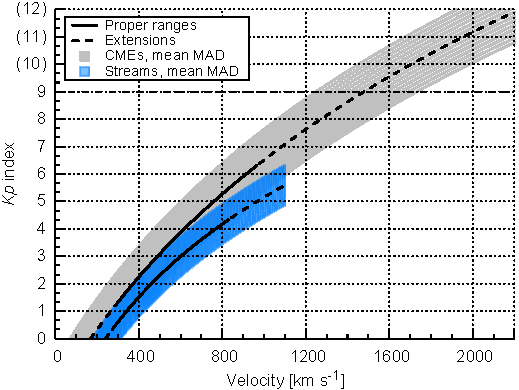
\includegraphics[width=0.6\textwidth]{figures_of_mine/chapter2/Kp_2dhistogram_V_sws123_fit_f3.pdf}
	}{
		\caption[\lofimage{figures_of_mine/chapter2/Kp_2dhistogram_V_sws123_fit_f3.pdf}I created the figure myself.]
		{Logarithmic fit curves for CMEs and streams with their proper ranges (solid lines) and extensions (dashed lines). The mean MAD bands corresponding to CMEs and streams are indicated by gray and blue shaded areas respectively. I extended the curve for CMEs up to a hypothetical \Kp{} of 12. The curve for solar wind streams is cut at \SI{1100}{\km\per\s} because streams do not occur at these high velocities. The curves are the same as in Figures~\ref{fig:Kp_2dhistogram_V_sws1_fit_e} and \ref{fig:Kp_2dhistogram_V_sws23_fit_e}.}
		\label{fig:Kp_2dhistogram_V_sws123_fit_f3}
	}
\end{figure}

The capped \Kp{} scale limits the capability to quantify the ground impacts of extremely fast CMEs. \Kp{} is linked to the \textit{ap}~index, which translates to the ground magnetic field disturbance at about \SI{+-50}{\degree} dipole latitudes and thus can directly be expressed in \si{\nano\tesla}. The limit could be overcome, if the fixed \Kp-to-\textit{ap} conversion table (see \autoref{tab:kp_to_ap_table}) would be redefined and extended above \Kp{} 9o. Then the absolute ground field disturbances evoked by extremely fast CMEs could be estimated via the \Kp{} relation for CMEs displayed in \autoref{fig:Kp_2dhistogram_V_sws123_fit_f3}.

% correlation studies between solar wind and geomagnetic indices, see Akasofu1981 p.~126, table\\


\section{Conclusions}
\label{sec:conclusions_ch2}
% summary
With the results presented in this chapter, I elaborate the step from solar wind properties to the prediction of their possible impact strength on the terrestrial magnetosphere. I derive empirical correlations and functional dependencies between solar wind properties and the geomagnetic \Kp~index, in order to obtain the capability to nowcast/forecast the \Kp~index. The following predictive models are obtained from the \Kp{} analyses in this chapter:
\begin{itemize*}
	\item The functional relation for the yearly \Kp{} averages relates \Kp{} with solar activity via the SSN, see Equation (\ref{eq:kp_ssn_relation}). The error to it is about 1/3~\Kp{}~unit, whereas seasonal variations further contribute up to 4/3~\Kp{}~units.
	\item The functional relation for enabling \Kp{} nowcasts relates \Kp{} with the solar wind electric field, see Equations~(\ref{eq:kpvsvbz_dependency_function_negative}) and (\ref{eq:kpvsvbz_dependency_function_positive}). Its MAD has a mean size of \SI{0.7}{\Kp}~units.
	\item The functional relation for enabling CME forecasts relates \Kp{} with the velocity of CME-associated flows, see Equation~(\ref{eq:kpvsv_CME_dependency_function}). Its MAD has a mean size of \SI{1.1}{\Kp}~units.
	\item The functional relation for enabling stream forecasts relates \Kp{} with the velocity of solar wind streams, see Equation~(\ref{eq:kpvsv_stream_dependency_function}). Its MAD has a mean size of \SI{0.7}{\Kp}~units.
\end{itemize*}

% Applications
The derived \Kp{} relations constitute a part of the CME forecast chain developed at the Institute for Astrophysics Göttingen. It consists of CME source region and coronal environment analysis, 3D modeling of the CME structure, CME acceleration and propagation modeling, CME arrival time and parameter prediction, and the subsequent forecast of relevant space weather effects, such as its impacts on the \Kp~index and on the ionospheric TEC.

Prototype \Kp{} relations were integrated into applications developed within the AFFECTS project (2011--2013). The following services contain early results from the present \Kp{} study and are accessible via the \mbox{AFFECTS} website\footnote{AFFECTS website: \urlfoot{http://www.affects-fp7.eu/services/}}. The corresponding services comprise a real-time plot, and alerts disseminated via RSS feeds and via mobile app. The \href{http://www.affects-fp7.eu/rssfeeds/ace_ap_forecast_plot/ace_realtime_ap_CH_GFT_plot.png}{Solar Wind and \Kp{} forecast plot} and the alerts are based on the \Kp--\vBz{} relation and process real-time solar wind measurements from L1: The \href{http://www.affects-fp7.eu/rssfeeds/rssfeed_kp/rssfeed_kp.xml}{L1 Kp Alert} is a threshold-based RSS feed that gets triggered when the estimated \Kp{} surpasses a threshold specified as being $7-$. The \href{http://www.affects-fp7.eu/rssfeeds/rssfeed_gnss/rssfeed_gnss.xml}{L1 GNSS Alert} and the \href{http://www.affects-fp7.eu/rssfeeds/rssfeed_aurora/rssfeed_aurora.xml}{L1 Aurora Alert} are threshold-based RSS feeds that derive GNSS error and auroral latitude from the \Kp{} estimate. The L1 Alerts are also accessible via the \href{https://itunes.apple.com/au/app/affects/id893579846}{AFFECTS app for iPhone}.\\
% 	\urltext{http://www.affects-fp7.eu/app-services/L1-Alerts/dataL1Alerts.txt}\\
% 	\item Android app L1 Alerts... \urltext{https://play.google.com/store/apps/details?id=com.afects.forecasts}


% conclusions from data processing
From the results presented in this study, I conclude that when correlating \vBz{} with \Kp{} it is of key importance to capture the 3"~hour minimum values, i.e., to use high resolution solar wind data, whereas when correlating velocity with \Kp{} the underlying data resolution is negligible. The results support that averaging over 3"~hour intervals neglects short-term geoeffective features in the magnetic field z"~component $B_\text{z}$. The calculation of 3"~hour minima considers these magnetic features and leads to a significant higher correlation with \Kp{}. \vBz{} is not well suited for remote forecast situations, because short-term variations in $B_\text{z}$ cannot be predicted yet, whereas the solar wind velocity is best suited for remote forecast situations.

% principal conclusions
There are differences in magnitude (more than 1~\Kp~unit) and trend in the \Kp--velocity prediction curves obtained from CMEs and streams. These significant differences confirm that it is beneficial to utilize separate relations for the prediction of \Kp{} from CME and stream velocities.

The \Kp--velocity dependency for CMEs is derived from velocity data of up to \SI{1100}{\km\per\s}. Assuming this relation holds true for higher speeds, the extension of it could be used to predict the \Kp{} impact of fast CMEs as well. Though, the \Kp--velocity relation for CMEs reaches the maximum \Kp{} of 9o at a CME velocity of \SI{1500}{\km\per\s}. The ground geomagnetic disturbances, generated by the rare, extremely fast CME events having velocities above this value, could be resolved and estimated via redefining and extending the conversion between the \Kp{} and \textit{ap} indices.

The examination of the prediction performance of the derived predictive models shows that strong geomagnetic storms exceeding a \Kp{} of 7 are being underestimated. The CME velocity relation underestimates their resulting actual \Kp{} on average by about 3~\Kp~units, whereas the stream velocity relation does not even reach the range of geomagnetic storms ($\text{\Kp} \geq 5$), that is, the stream velocity relation is good in predicting lower geomagnetic activity but is not able to predict storms.

As the obtained functional relations are based only on one or two aspects of the solar wind--magnetosphere coupling, they cannot compete with full-fledged solar wind coupling functions, such as the rate magnetic flux is opened at the magnetopause (\autoref{eq:newell_merging_function}), nor with current prediction models based on artificial neural networks or \Kp{} persistence. Nevertheless, they enable empirical estimations of the mean geomagnetic activity impact for special forecast situations, that is, \Kp{} can directly be quantified from measured solar activity, monitored in-situ solar wind, and remotely determined CME and stream velocities.

% discuss $r_{vB_\text{z}} = -0.72$ vs $r_{d\phi/dt} = 0.76$ (Newell)\\


\bigskip
{\small
\noindent \textit{Acknowledgments.} Part of the research leading to the results presented in this chapter has received funding from the EU~FP7 project AFFECTS under grant 263506.
The analyses in this chapter rely on the \Kp~index, calculated and made available by the GFZ~Potsdam from data collected at magnetic observatories. Thank goes to the involved national institutes, the INTERMAGNET network and ISGI (\urltext{isgi.unistra.fr}). The author thanks the WDC-SILSO at the SIDC (ROB) for maintaining and providing the international sunspot number series. Additional thank goes to the OMNI PIs/teams for creating and making available the solar wind in-situ data. The OMNI data are supplied by the SPDF at the GSFC (NASA). The hourly SWS list, updated until the end of 2016, was kindly provided by Ian~Richardson of the GSFC and CRESST/University of Maryland.
}

